% Reporte del Data Challenge – Mundial 2026, equipo 5.
% Compilar desde esta carpeta:   tectonic -X compile reporte.tex
% Las figuras se leen de ../../output/figures/ y las tablas de ../../output/tables/rep_*.tex;
% las generan los scripts de code/ (las tablas, code/09_figuras_reporte.py). No editarlas aquí.
\documentclass[11pt,letterpaper]{article}
\usepackage{fontspec}
\setmainfont{texgyretermes}[Extension=.otf, UprightFont=*-regular, BoldFont=*-bold,
  ItalicFont=*-italic, BoldItalicFont=*-bolditalic]
\usepackage[spanish,es-noshorthands,es-nodecimaldot,es-tabla]{babel}
\usepackage[margin=1.8cm,top=1.6cm,bottom=1.7cm]{geometry}
\usepackage{amsmath,booktabs,graphicx,tabularx,xcolor,enumitem,caption,float}
\usepackage[hidelinks]{hyperref}
\graphicspath{{../../output/figures/}}
\setlength{\parskip}{3pt}
\setlength{\parindent}{0pt}
\setlist{nosep,leftmargin=1.2em}
\captionsetup{font=small,labelfont=bf,skip=3pt}
\newcommand{\completar}[1]{\textcolor{red}{[#1]}}
\newcommand{\seccion}[1]{\vspace{4pt}{\large\bfseries #1}\par\vspace{1pt}}

\begin{document}

\begin{center}
{\LARGE\bfseries ¿El Mundial encareció lo que se consume con el futbol?}\\[3pt]
{\large Precios de productos complementarios en las ciudades sede del Mundial 2026}\\[5pt]
Data Challenge -- Mundial 2026 \textbullet{} Equipo 5: Diego Méndez, André Herrera y Luis Victoria\\
Microeconometría Aplicada / Inferencia Causal, ITAM \textbullet{} 2 de diciembre de 2026\\
Repositorio: \completar{liga de GitHub}
\end{center}

\vspace{4pt}
\seccion{Resumen ejecutivo}

\textbf{Pregunta.} ¿Cuánto subieron, por el Mundial, los precios de los bienes y servicios que
se consumen junto con el futbol (sin hospedaje) en Ciudad de México, Guadalajara y Monterrey
durante las quincenas con partidos (11 de junio al 5 de julio de 2026)?

\textbf{Cómo lo medimos.} Con el Índice Nacional de Precios al Consumidor (INPC) por ciudad de
INEGI estimamos una diferencia en diferencias: comparamos el cambio de precio de 14 productos
complementarios en las 3 sedes contra el de las otras 52 ciudades del INPC, con efectos fijos
ciudad$\times$producto y producto$\times$quincena. Como solo hay 3 ciudades tratadas, la
inferencia es por permutación de sedes (Fisher; Conley y Taber). Una segunda fuente, los precios
por tienda de PROFECO, mide el mismo producto en la misma tienda y su distancia al estadio.

\textbf{Resultados principales.}
\begin{enumerate}
\item \textbf{Los servicios subieron.} En el grupo de servicios (comida fuera de casa, transporte
  y centros nocturnos), los precios subieron \textbf{1.8\%} más en las sedes durante el torneo
  (IC 95\%: $-0.3$ a 3.8; $p=0.10$). En un verano normal los servicios de las sedes se quedan atrás del resto del país;
  al descontar esa estacionalidad (triple diferencia), el efecto es \textbf{2.8\%} (IC 95\%: 0.2
  a 5.3; $p=0.03$). Equivale a unos 3.5 meses de inflación normal de servicios concentrados en
  seis semanas. El alza viene de estacionamiento (+4.0\%), autobús foráneo (+2.6\%) y centros
  nocturnos (+1.9\%); restaurantes y fondas no cambiaron.
\item \textbf{Los bienes de tienda no subieron.} Cerveza, refrescos, botanas y pantallas: $-0.6\%$
  en el INPC ($p=0.67$). Con PROFECO (mismo producto, misma tienda): +0.2\% (IC 95\%: $-0.4$ a
  0.8), lo que descarta alzas mayores a 0.8\%. Tampoco subieron en las tiendas a menos de 5 km del
  estadio o del Fan Fest.
\item \textbf{Por qué: los precios de los bienes los fija la cadena, no la tienda.} Dentro de la
  misma cadena y producto, las tiendas de las sedes no son más caras que las del resto del país
  (diferencia mediana: 0.0\%). La cadena explica 62\% de la dispersión del precio entre tiendas;
  la ciudad, 31\%.
\item \textbf{Tampoco hubo un alza nacional.} Frente a los mismos meses de 2018--2025, los
  complementarios no subieron en todo el país durante el torneo; los licores incluso bajaron
  cerca de 3\% (lo muestran el INPC y PROFECO por separado).
\end{enumerate}

\textbf{Conclusión.} El Mundial funcionó como un choque de demanda local y temporal. Encareció los
servicios cuya capacidad no crece en semanas y cuyo precio se decide localmente (lugares de
estacionamiento, asientos de autobús, centros nocturnos), pero no los bienes que venden cadenas
nacionales con precios regionales. Los efectos son moderados y se estiman con imprecisión: con 3
sedes solo podemos detectar alzas de ${\sim}3\%$ en servicios y ${\sim}0.9\%$ en bienes. Además,
los datos promedian toda la zona metropolitana y toda la quincena, así que un alza junto al
estadio o solo en días de partido aparece diluida: nuestras cifras son una cota inferior del
efecto local.

\newpage
\seccion{(a) Pregunta}
¿Cuál fue el efecto causal del Mundial sobre los precios de los productos complementarios al
futbol en las tres ciudades sede, durante las quincenas con partidos? Llamamos
\emph{complementarios} a lo que se consume más cuando se ve o se asiste a un partido: comer y beber
fuera de casa (loncherías y fondas, restaurantes, pizzas, centros nocturnos), moverse
(taxi, estacionamiento, autobús foráneo, avión), y ver o jugar en casa (cerveza, refrescos, papas,
botanas, televisores, artículos deportivos). Hoteles y paquetes turísticos quedan fuera, como pide
la consigna. Además preguntamos: ¿el efecto difiere entre servicios locales y bienes comerciables?
¿se concentra cerca de los estadios? El torneo es un buen experimento: México se eligió como sede
en 2018 y las ciudades en 2022, por razones ajenas al mercado local de estos productos.

\seccion{(b) Datos}
\begin{center}
\footnotesize
\begin{tabularx}{\textwidth}{@{}p{2.2cm}XX@{}}
\toprule
& \textbf{Principal: INPC por ciudad (INEGI)} & \textbf{Segunda fuente: Quién es Quién en los Precios (PROFECO)} \\
\midrule
Quién lo recaba & INEGI, con precios de una muestra fija de establecimientos en cada ciudad & PROFECO, con visitas a supermercados, tiendas de conveniencia y departamentales \\
Periodo & 1Q ene 2018 a 2Q oct 2026 (212 quincenas); estimación desde 1Q ene 2025 & 24 quincenas entre ene 2025 y jul 2026 (no hay feb--abr ni ago 2026) \\
Unidad & Índice (base 2Q jul 2018 = 100) de un producto genérico en una ciudad y quincena & Precio en pesos de un producto (marca y presentación) en una tienda; lo promediamos por quincena \\
Población & Consumo de los hogares urbanos de 55 ciudades (canasta y ponderadores 2024) & 651 tiendas (276 en sedes) y 691 productos; tiendas de cadena en ciudades grandes \\
Virtudes & Oficial y pública; quincenal; 52 ciudades de control; 8 años de historia; incluye servicios & Mismo producto en la misma tienda; coordenadas de cada tienda; permite comparar cadenas \\
Limitaciones & Promedia toda la zona metropolitana; es un índice; sin ventas ni boletos & Sin servicios; pocas tiendas en Guadalajara (26) y Monterrey (27); solo dos años \\
\bottomrule
\end{tabularx}
\end{center}
\vspace{-4pt}
Ninguna de las dos fuentes trae ventas; la consigna pide precios \emph{y/o} ventas, así que
trabajamos con precios. Las encuestas de INEGI con ventas (EMEC, EMS) solo están por estado y
mezclan restaurantes con hoteles.

\seccion{(c) Ecuación}
Sea $y_{cjt} = 100\cdot\ln(\text{índice})$ del producto genérico $j$ en la ciudad $c$ y la quincena $t$:
\begin{equation}
y_{cjt} = \alpha_{cj} + \delta_{jt} + \beta\,(\text{Sede}_c \times \text{Mundial}_t) + \gamma\,(\text{Sede}_c \times \text{Después}_t) + \varepsilon_{cjt}
\end{equation}
\begin{itemize}
\item $\alpha_{cj}$: efecto fijo ciudad$\times$producto (por ejemplo, el estacionamiento es más caro en CDMX).
\item $\delta_{jt}$: efecto fijo producto$\times$quincena; absorbe lo que le pasa a cada producto en
  todo el país: inflación, el aumento del IEPS a refrescos en enero de 2026, vacaciones y temporada.
\item $\text{Sede}_c = 1$ para CDMX, Guadalajara y Monterrey. $\text{Mundial}_t = 1$ en la 1Q y 2Q
  de junio y la 1Q de julio de 2026, las quincenas con los 13 partidos en México.
  $\text{Después}_t = 1$ de la 2Q de julio a la 2Q de octubre de 2026.
\item \textbf{$\boldsymbol\beta$ es el parámetro de interés}: cuánto más (en \%) cambiaron los
  precios en las sedes durante el torneo que en las otras 52 ciudades, frente a ene 2025--may
  2026. Es el efecto promedio sobre las tres sedes tratadas. $\gamma$ mide si el alza se quedó
  después.
\end{itemize}
Se estima por separado para servicios, bienes comerciables y placebos (tortilla, detergentes,
analgésicos, pañales, consulta médica, mantenimiento de auto). El estudio de evento cambia
$\beta$ y $\gamma$ por un coeficiente por quincena, con la 2Q de mayo de 2026 como referencia.
\textbf{Inferencia:} con 3 ciudades tratadas, el error agrupado por ciudad no es confiable (da
$p=0.02$ en servicios). Reportamos el $p$ de la permutación exacta de Fisher (se asigna ``sede'' a
las 26,235 tripletas posibles de ciudades) y el intervalo de Conley y Taber (con las 22,100
tripletas de ciudades de control). Con PROFECO, la ecuación es la misma con tienda$\times$producto
y producto$\times$quincena como efectos fijos, comparando mayo con las quincenas del torneo.

\newpage
\seccion{(d) Resultados principales}
\begin{figure}[H]
\centering
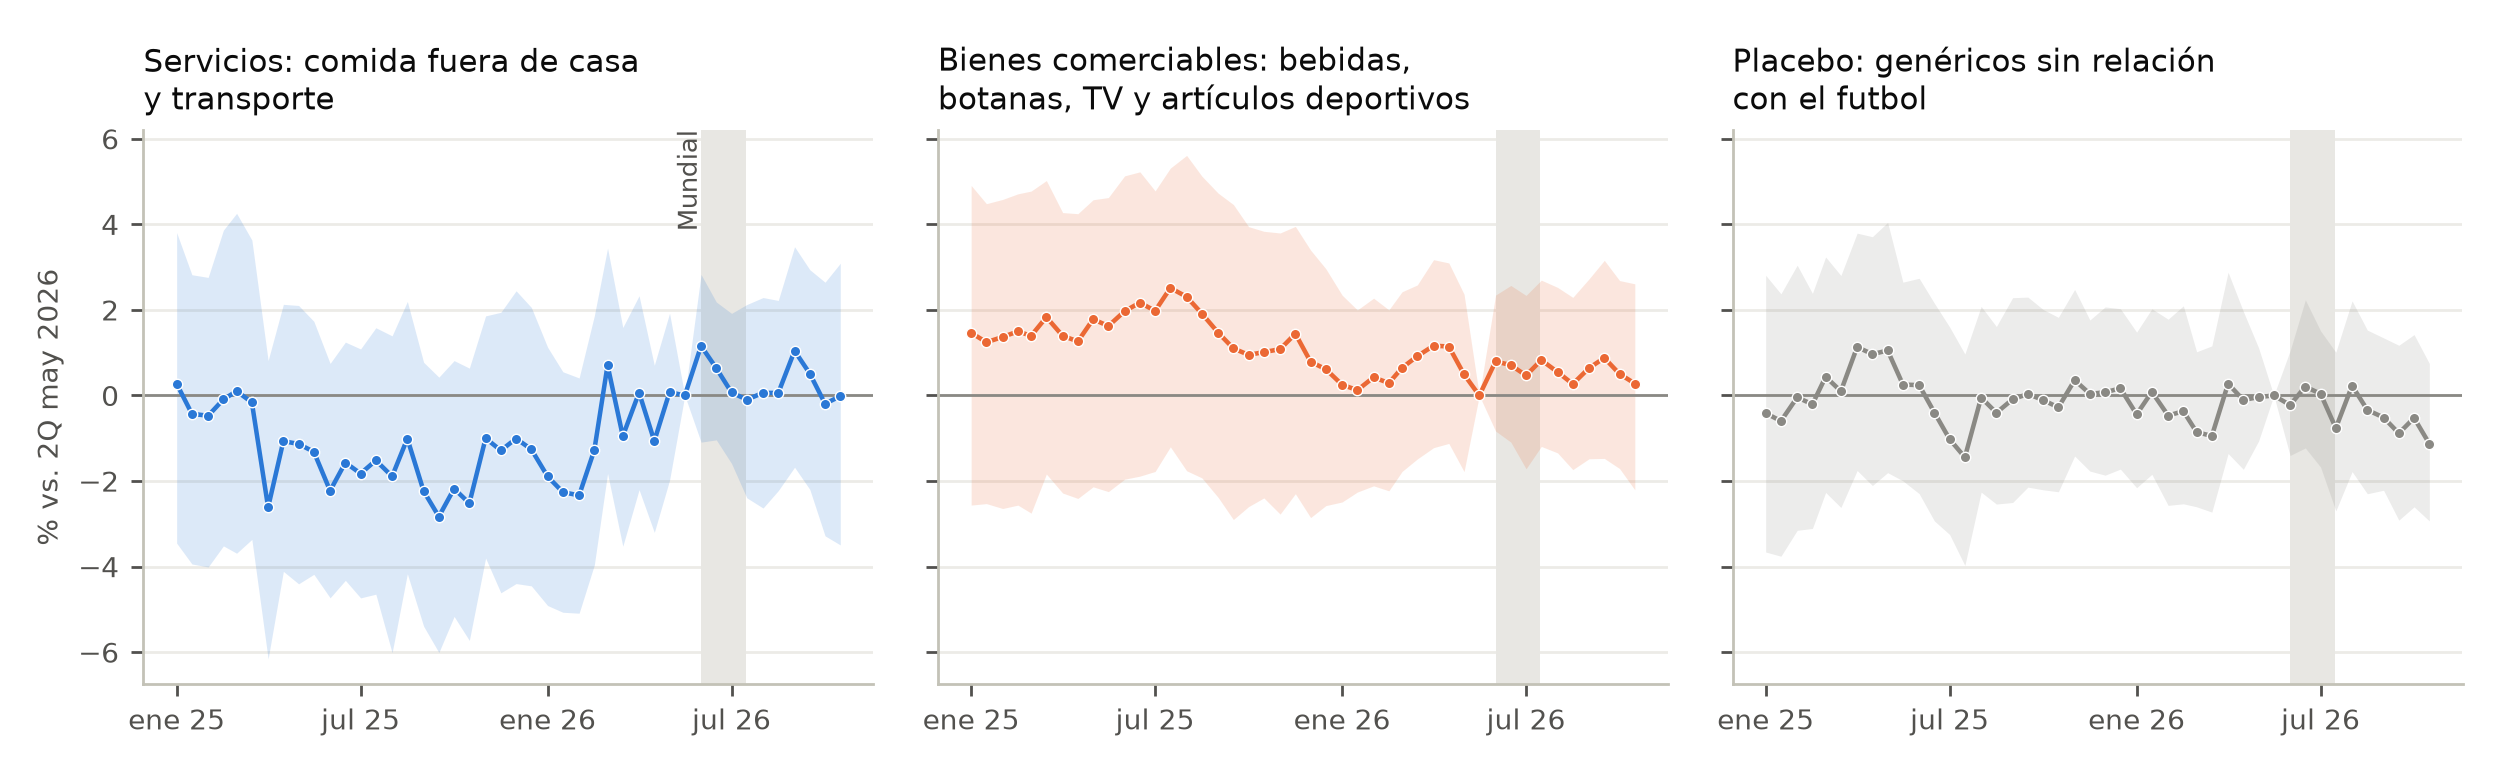
\includegraphics[width=\textwidth]{rep_estudio_evento.png}
\caption{Estudio de evento (INPC): diferencia entre sedes y no sedes por quincena, relativa a la 2Q
de mayo de 2026. Banda: IC 95\% de Conley y Taber. Franja gris: quincenas con partidos.}
\end{figure}
\begin{table}[H]
\centering\footnotesize
\caption{Efecto del Mundial sobre los precios en las sedes (\%). IC 95\% de Conley y Taber; $p$ por permutación de sedes.}
% Generado por code/09_figuras_reporte.py; no editar a mano.
\begin{tabular}{@{}lrcrrr@{}}
\toprule
& \multicolumn{3}{c}{Durante el Mundial ($\beta$)} & \multicolumn{2}{c}{Después ($\gamma$)} \\
\cmidrule(lr){2-4}\cmidrule(l){5-6}
Grupo & $\beta$ & IC 95\% & $p$ & $\gamma$ & $p$ \\
\midrule
\multicolumn{6}{@{}l}{\emph{INPC: 3 sedes contra 52 ciudades}} \\
Servicios (comida fuera de casa y transporte) & 1.80 & [$-0.35$, 3.83] & 0.10 & 1.38 & 0.25 \\
Bienes comerciables & $-0.57$ & [$-2.78$, 2.25] & 0.67 & $-0.66$ & 0.61 \\
Todos los complementarios & 0.79 & [$-0.66$, 2.52] & 0.32 & 0.50 & 0.54 \\
Placebo & 0.10 & [$-1.81$, 1.79] & 0.92 & $-0.47$ & 0.60 \\
\multicolumn{6}{@{}l}{\emph{PROFECO: mismo producto en la misma tienda, mayo contra el torneo}} \\
Cerveza, refrescos, agua, botanas, licores y pollo & 0.19 & [$-0.44$, 0.75] & 0.54 & 0.31 & 0.34 \\
Placebo (detergentes, papel, aceite, arroz, leche) & 0.22 & [$-0.34$, 0.83] & 0.39 & 0.02 & 0.96 \\
\bottomrule
\end{tabular}

\end{table}

\textbf{Tamaño del efecto.} Un alza de 1.8\% en servicios es moderada pero no trivial: en 2025 los
servicios de las ciudades que no son sede subieron 0.25\% por quincena, así que el Mundial
equivale a unos 3.5 meses de inflación normal concentrados en seis semanas. En pesos, es como
pagar \$90 en vez de \$88 por un estacionamiento. El estudio de evento muestra que el alza empieza
en marzo de 2026, antes del torneo, sube en la primera quincena de junio y se queda después
($\gamma=1.4$): los precios de servicios cambian poco y en escalones, no en picos. En bienes, el
intervalo de PROFECO descarta alzas mayores a 0.8\%.

\textbf{Qué tan generalizable es.} $\beta$ es el efecto promedio en tres zonas metropolitanas grandes
que ya recibían turismo, medido con la muestra fija de establecimientos de INEGI repartida en toda
la ciudad. Por eso es una \emph{cota inferior} de lo que pasó cerca de los estadios o en días de
partido. Aplica a megaeventos en ciudades grandes; en una ciudad pequeña el mismo número de
visitantes sería un choque mayor. No aplica a bienes que venden cadenas nacionales.

\seccion{(e) Supuestos, en este contexto}
\begin{enumerate}
\item \textbf{Sin Mundial, los servicios de las sedes habrían seguido a los del resto del país.}
  Es decir: entre ene 2025--may 2026 y jun--jul 2026, el estacionamiento, el autobús foráneo o los
  centros nocturnos en CDMX, Guadalajara y Monterrey habrían cambiado igual que en las otras 52
  ciudades. No hay diferencias antes del torneo (prueba conjunta del estudio de evento: $p=0.37$
  en servicios, 0.39 en bienes, 0.94 en placebos). \textbf{La amenaza es la temporada de verano}:
  en destinos de playa (Cancún, Acapulco, La Paz) los servicios suben más en verano que en las
  grandes ciudades. En 2018--2025, los servicios de las sedes \emph{siempre} se quedaron atrás en
  junio--julio ($-0.7$ puntos en promedio). Si eso pasó en 2026, $\beta$ \emph{subestima} el
  efecto. Por eso hacemos la triple diferencia (sección f).
\item \textbf{Anticipación.} Las fechas se conocían desde años antes, así que los negocios podían
  subir precios antes del torneo, y el estudio de evento muestra un escalón en marzo de 2026. Con
  la comparación contra ene 2025--may 2026, $\beta$ incluye ese escalón (efecto total); contra
  mar--may 2026 solo mide el salto durante los partidos (0.8\%).
\item \textbf{Sin contagio a las ciudades de control.} Aficionados pudieron alojarse o pasear en
  ciudades cercanas (Toluca, Cuernavaca, Pachuca, Saltillo), y los partidos de México se vieron en
  todo el país. Ambas cosas sesgarían $\beta$ hacia cero. Excluimos las ciudades vecinas y
  revisamos si hubo un alza nacional (sección f): no la hubo.
\item \textbf{Ningún otro choque exclusivo de las sedes en esas quincenas.} Los choques nacionales
  (como el IEPS a refrescos de enero de 2026) los absorbe $\delta_{jt}$; los productos placebo, que
  no deberían responder al futbol, tampoco se mueven.
\item \textbf{Composición estable.} El INPC sigue los mismos establecimientos y la canasta 2024 ya
  estaba vigente desde 2024; PROFECO compara el mismo producto en la misma tienda.
\end{enumerate}

\seccion{(f) Robustez y heterogeneidad}
\begin{figure}[H]
\centering
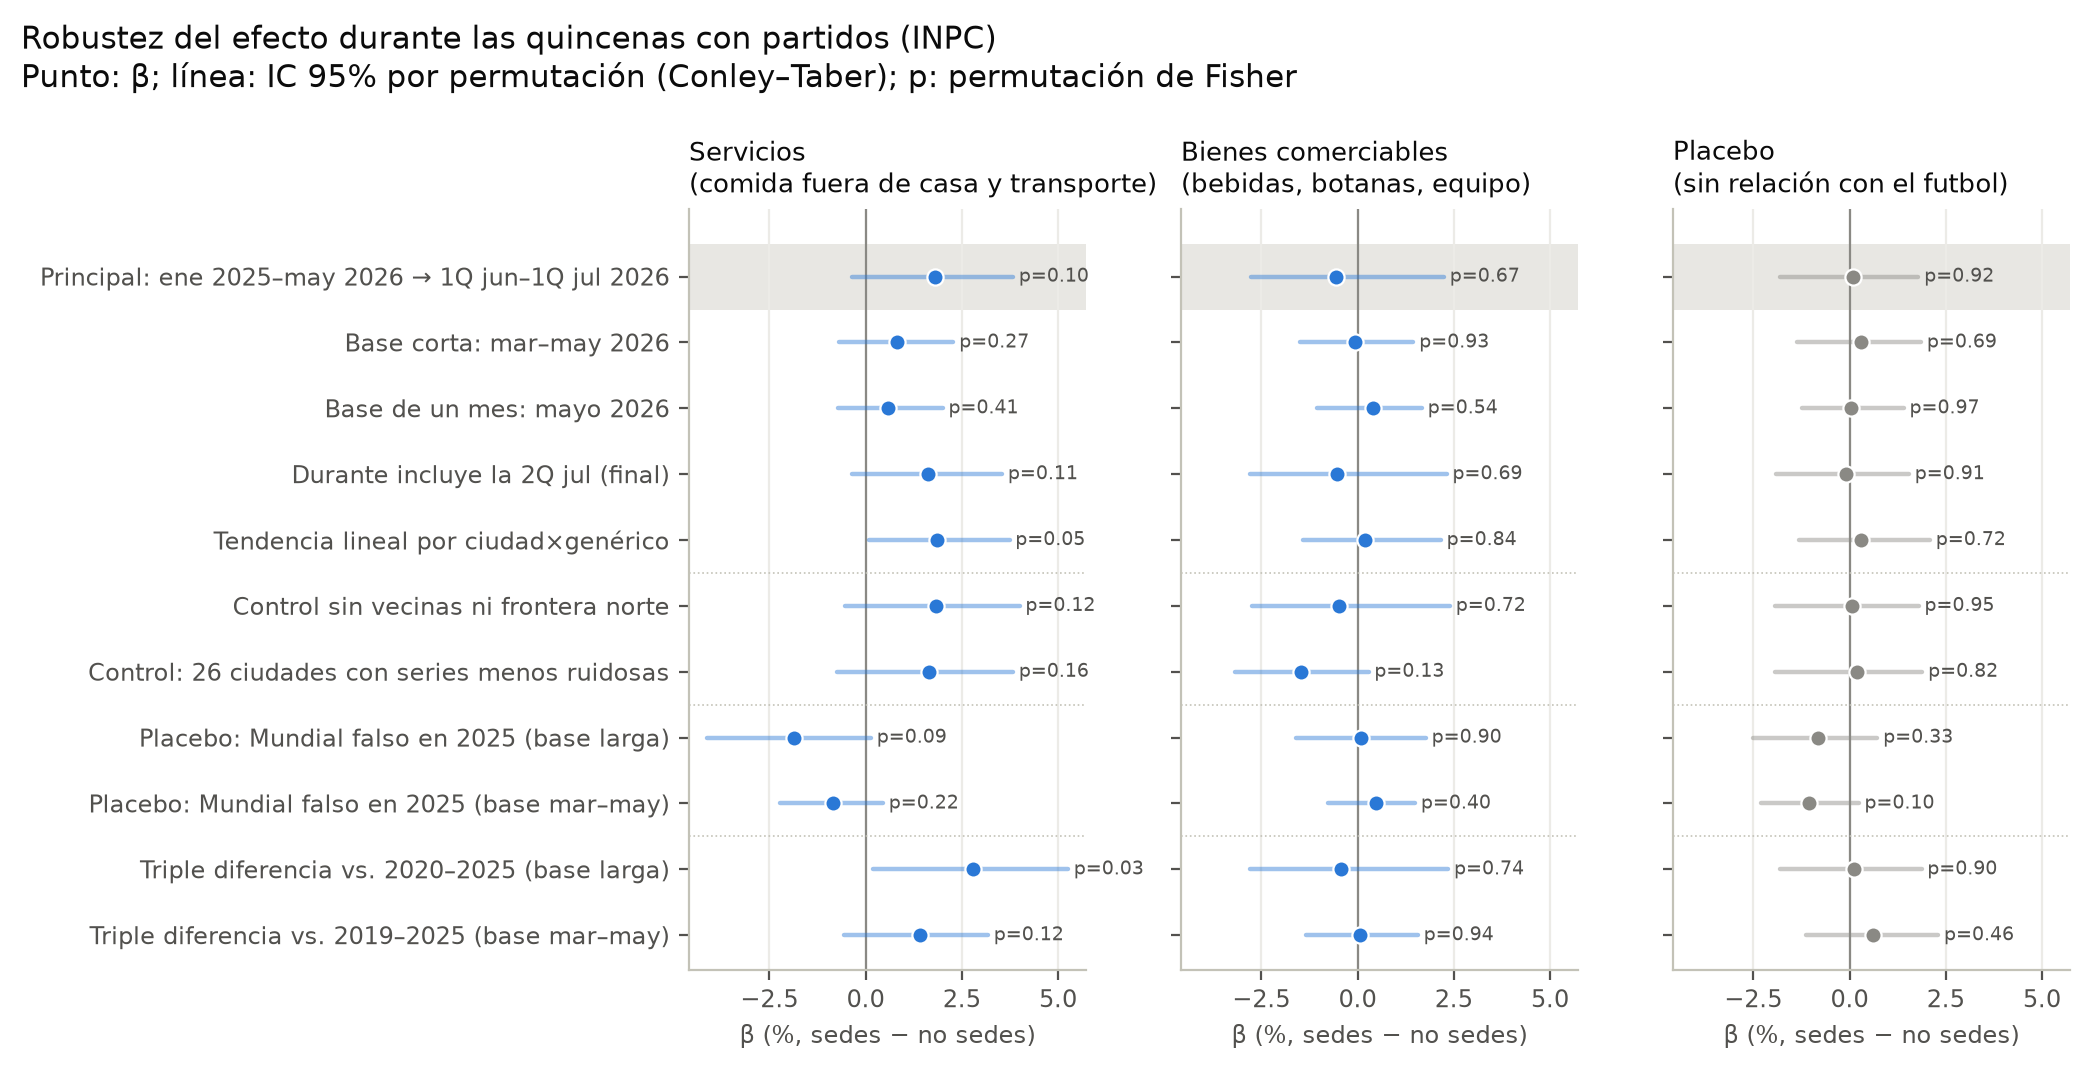
\includegraphics[width=0.93\textwidth]{fig_robustez.png}
\caption{Robustez de $\beta$ (INPC). Cada fila cambia una sola cosa del diseño principal (fila sombreada).}
\end{figure}
\textbf{Robustez.} Elegimos como prueba principal la \textbf{triple diferencia}: el cambio de 2026
menos el cambio promedio de los mismos meses en 2020--2025. La elegimos porque responde a la
amenaza que encontramos en los datos (la estacionalidad y la tendencia propias de las sedes). Da
\textbf{+2.8\%} en servicios (IC 95\%: 0.2 a 5.3; $p=0.03$), y 0.1\% ($p=0.90$) en placebos. El
placebo de un ``Mundial falso'' en 2025 confirma la amenaza: da $-1.9\%$ ($p=0.09$), es decir, en un
año normal las sedes se quedan atrás. El resto de las variantes (tendencias lineales por
ciudad$\times$producto, sin ciudades vecinas ni fronterizas, controles menos ruidosos, incluir la
final) dan entre +1.6\% y +1.9\%. Con la comparación contra mar--may o solo mayo, el efecto baja a
0.6--0.8\% porque esa base ya incluye el escalón de marzo. Con PROFECO, 14 variantes dan cero en
bienes. Por último, la \textbf{prueba nacional} (2026 contra 2018--2025, en 275 genéricos) no
encuentra un alza de los complementarios en todo el país ($-0.5$ puntos en bienes, $p=0.22$).

\textbf{Heterogeneidad (justificación teórica).} Un choque de demanda temporal y local sube el
precio cuando (i) la oferta no puede crecer en semanas, (ii) el precio se fija localmente y (iii)
el comprador, un visitante, compara poco. Los servicios cumplen las tres; los bienes empacados no:
se resurten en días y su precio lo fija la cadena por región. La Tabla 2 confirma la predicción y
la afina: el alza está en los servicios con capacidad fija (estacionamientos, asientos de autobús,
centros nocturnos), no en restaurantes y fondas, que son muchos y fijan sus precios en menús que
cambian poco. PROFECO muestra el mecanismo: dentro de la misma cadena, las sedes no son más caras.

\begin{table}[H]
\centering\footnotesize
\caption{Heterogeneidad del efecto durante el Mundial (\%). IC 95\% de Conley y Taber; $p$ por permutación.}
% Generado por code/09_figuras_reporte.py; no editar a mano.
\begin{tabular}{@{}llrcr@{}}
\toprule
Dimensión & Grupo & Efecto & IC 95\% & $p$ \\
\midrule
Tipo de producto (INPC) & Servicios sin transporte aéreo & 1.10 & [$-0.10$, 2.13] & 0.06 \\
 & Bienes comerciables & $-0.57$ & [$-2.78$, 2.25] & 0.67 \\
Servicios por producto (INPC) & Estacionamiento & 3.95 & [$-1.53$, 8.09] & 0.11 \\
 & Autobús foráneo & 2.55 & [$-0.69$, 7.67] & 0.19 \\
 & Servicios recreativos y centros nocturnos & 1.91 & [$-2.78$, 4.95] & 0.24 \\
 & Restaurantes & $-0.41$ & [$-2.16$, 1.17] & 0.61 \\
 & Loncherías, fondas y taquerías & $-0.36$ & [$-2.49$, 1.69] & 0.73 \\
Sede (INPC, complementarios) & Guadalajara / Monterrey / CDMX & 2.29 / 0.60 / $-0.52$ &  & 0.13 / 0.60 / 0.66 \\
Cercanía (PROFECO, bienes) & A $\le$5 km del estadio o Fan Fest, menos el resto & $-0.37$ &  & 0.50 \\
Mecanismo (PROFECO) & Precio sede $-$ resto, misma cadena y producto & mediana 0.0 &  &  \\
\bottomrule
\end{tabular}

\end{table}

\seccion{(g) Conclusiones}
Nuestra métrica dice que el Mundial sí movió precios, pero solo donde la teoría lo predice: los
servicios locales con capacidad fija subieron entre 1.8\% y 2.8\% en las sedes, mientras que los
bienes de tienda no se movieron ni en las sedes, ni cerca de los estadios, ni en el resto del país.
\textbf{Fortalezas:} dos fuentes independientes que coinciden; inferencia adecuada para 3 ciudades
tratadas; placebos de producto y de año; una triple diferencia que corrige la estacionalidad
propia de las sedes; y un mecanismo medido en los datos. \textbf{Limitaciones:} con 3 sedes el
efecto en servicios es impreciso (solo detectamos alzas de ${\sim}3\%$), y su tamaño depende de si
el escalón de marzo de 2026 se atribuye al torneo; los datos promedian toda la ciudad y la
quincena, así que no ven el alza junto al estadio ni en días de partido (lo más probable es que
ahí haya sido mayor); no hay ventas ni precios dentro de los estadios; y PROFECO tiene pocas
tiendas en Guadalajara y Monterrey.

\seccion{(h) Uso de IA y contribución de cada miembro}
\textbf{Uso de IA.} Usamos Claude (Anthropic), a través de Claude Code, para ubicar las fuentes de
datos (INEGI y PROFECO), escribir el código en Python de descarga, limpieza, estimación y
gráficas, proponer el diseño de la estimación y de las pruebas de robustez, y redactar un primer
borrador de este reporte. \completar{Describir cómo revisó y validó el equipo el código, los
resultados y el texto.}

\textbf{Contribuciones.} Diego Méndez: \completar{completar}. André Herrera: \completar{completar}.
Luis Victoria: \completar{completar}. \completar{Indicar si algún miembro acepta una deducción.}

\end{document}
